%% fig02-linear-interpolation, caption is in docs/figures/README.md
\documentclass[border=8pt]{standalone}
% Shared preamble for the interpolation-geometry figures.
% \input by every figNN-*.tex. 
\usepackage[T1]{fontenc}
\usepackage{amsmath,amssymb}
\usepackage{tikz}
\usetikzlibrary{shapes.misc,arrows.meta,calc,decorations.pathreplacing,positioning,fit,backgrounds}

\definecolor{ink}{HTML}{1A1A1A}
\definecolor{gridc}{HTML}{9AA3AD}
\definecolor{accent}{HTML}{1F5FA9}
\definecolor{good}{HTML}{2E7D4F}
\definecolor{bad}{HTML}{B03030}
\definecolor{soft}{HTML}{E6EDF7}
\definecolor{softg}{HTML}{E3F0E8}
\definecolor{softr}{HTML}{F8E6E6}
\definecolor{amber}{HTML}{B8860B}


\tikzset{
  gpt/.style={circle,fill=ink,inner sep=1.15pt},
  ghost/.style={circle,draw=gridc,fill=white,inner sep=1.15pt},
  dep/.style={cross out,draw=accent,thick,inner sep=1.6pt,minimum size=4pt},
  traj/.style={gridc,dotted,thick,-{Stealth[length=2mm]}},
  htraj/.style={accent,very thick,-{Stealth[length=2.6mm]}},
  lbl/.style={font=\footnotesize},
  slbl/.style={font=\scriptsize},
}

\begin{document}
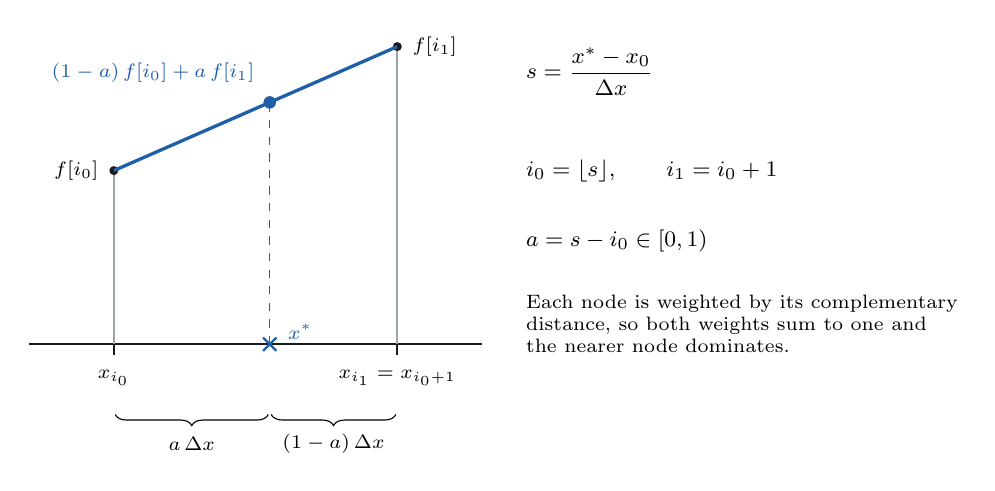
\begin{tikzpicture}[x=3.6cm,y=1.05cm]
  \pgfmathsetmacro{\aa}{0.55}
  \pgfmathsetmacro{\fz}{2.1}
  \pgfmathsetmacro{\fo}{3.6}
  \pgfmathsetmacro{\fs}{\fz+\aa*(\fo-\fz)}
  \draw[ink,thick] (-0.3,0) -- (1.3,0);
  \foreach \i in {0,1} \draw[ink,thick] (\i,-0.13) -- (\i,0.13);
  \draw[gridc,thick] (0,0) -- (0,\fz);
  \draw[gridc,thick] (1,0) -- (1,\fo);
  \node[gpt] at (0,\fz) {};
  \node[gpt] at (1,\fo) {};
  \node[slbl,anchor=east] at (-0.02,\fz) {$f[i_0]$};
  \node[slbl,anchor=west] at (1.02,\fo) {$f[i_1]$};
  \draw[accent,very thick] (0,\fz) -- (1,\fo);
  \draw[accent,dashed] (\aa,0) -- (\aa,\fs);
  \node[circle,fill=accent,inner sep=1.6pt] at (\aa,\fs) {};
  \node[slbl,accent,anchor=south east] at (\aa-0.02,\fs+0.12) {$(1-a)\,f[i_0]+a\,f[i_1]$};
  \node[dep] at (\aa,0) {};
  \node[slbl,accent,anchor=west] at (\aa+0.03,0.15) {$x^{*}$};
  \node[slbl,anchor=north] at (0,-0.2) {$x_{i_0}$};
  \node[slbl,anchor=north] at (1,-0.2) {$x_{i_1}=x_{i_0+1}$};
  \draw[decorate,decoration={brace,amplitude=4pt,mirror}] (0.005,-0.85) -- (\aa-0.005,-0.85);
  \node[slbl] at (\aa/2,-1.2) {$a\,\Delta x$};
  \draw[decorate,decoration={brace,amplitude=4pt,mirror}] (\aa+0.005,-0.85) -- (0.995,-0.85);
  \node[slbl] at ({(\aa+1)/2},-1.2) {$(1-a)\,\Delta x$};
  \node[lbl,anchor=west] at (1.42,3.3) {$s=\dfrac{x^{*}-x_0}{\Delta x}$};
  \node[lbl,anchor=west] at (1.42,2.1) {$i_0=\lfloor s\rfloor,\qquad i_1=i_0+1$};
  \node[lbl,anchor=west] at (1.42,1.25) {$a=s-i_0\in[0,1)$};
  \node[slbl,anchor=west,align=left] at (1.42,0.25)
    {Each node is weighted by its complementary\\ distance, so both weights sum to one and\\
     the nearer node dominates.};
\end{tikzpicture}
\end{document}
